%%%%%%%%%%%%%%%%%%%%%%%%%%%%%%%%%%%%%%%%%%%%%%%%%%%%%%%%%%%%%%%%%%%%%%%%%%%

\documentclass{standalone}

\usepackage{mathptmx}
\usepackage{tikz}
\usetikzlibrary{external}
\tikzexternalize{circle-hexagon}

%% We default to Times.
\renewcommand{\rmdefault}{ptm}
\renewcommand{\ttdefault}{pcr}
%% Enable Times/Palatino main text font.
\normalfont\selectfont

\newcommand{\comma}{,\,}
\newcommand{\tuple}[2]{\left({#1}\comma {#2}\right)}

%% A general circle.
\newcommand{\myCircle}{%%
  %% Draw the circle.
  \draw[lineStyle] (centre) circle[radius=\radius];
  %% Label the centre of the circle.
  \node[nodeStyle] at (centre) {};
  \node at (centre) [below] {$\tuple{0}{0}$};
}

%% A hexagon that is inscribed inside a unit circle.
\newcommand{\myHexagon}{%%
  %% Draw the inscribed hexagon.
  \draw[lineStyle] (A) -- (B) -- (C) -- (D) -- (E) -- (F) -- cycle;
  %% Label the corners where the hexagon touches the circle.
  \xyPoint{A}{\tuple{1}{0}}{right}
  \xyPoint{B}{\tuple{\frac{1}{2}}{\frac{\sqrt{3}}{2}}}{above right}
  \xyPoint{C}{\tuple{-\frac{1}{2}}{\frac{\sqrt{3}}{2}}}{above left}
  \xyPoint{D}{\tuple{-1}{0}}{left}
  \xyPoint{E}{\tuple{-\frac{1}{2}}{-\frac{\sqrt{3}}{2}}}{below left}
  \xyPoint{F}{\tuple{\frac{1}{2}}{-\frac{\sqrt{3}}{2}}}{below right}
}

%% Label a point.
%%
%% #1 -- The coordinates of the point.
%% #2 -- Label the point with this name.
%% #3 -- Where to position the label.
\newcommand{\xyPoint}[3]{%%
  \node[nodeStyle] at (#1) {};
  \node at (#1) [#3] {$#2$};
}

%% A unit circle with an inscribed hexagon.

\begin{document}

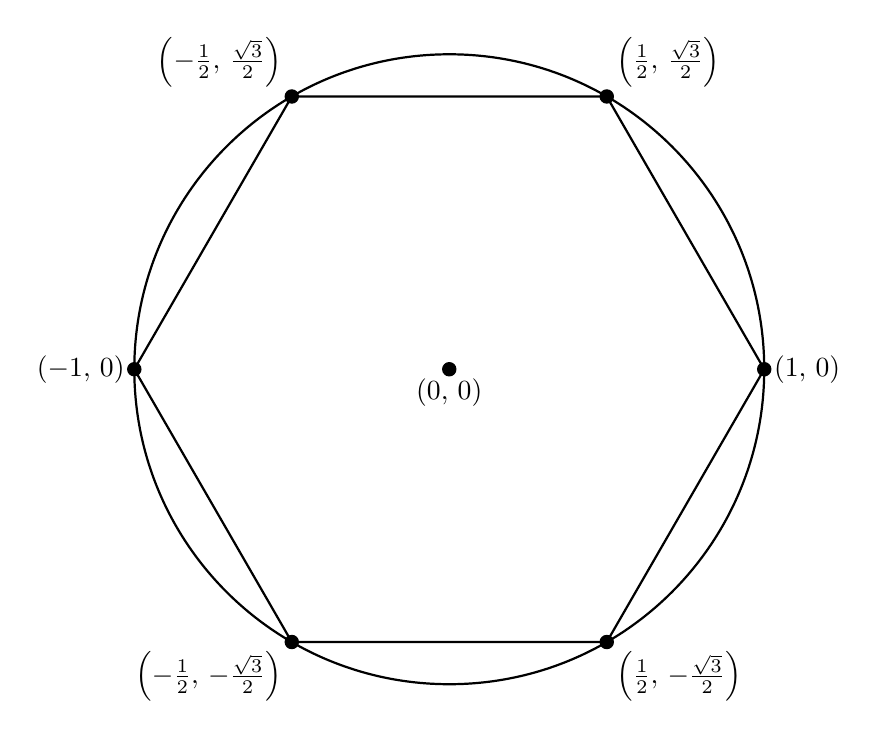
\begin{tikzpicture}[%%
  lineStyle/.style={-,thick},%%
  nodeStyle/.style={draw,inner sep=1.7pt,circle,fill=black,black}
]
%%
%%
\pgfmathsetmacro{\radius}{4}
\pgfmathsetmacro{\dx}{\radius}
\pgfmathsetmacro{\xlow}{0}
\pgfmathsetmacro{\ylow}{0}
\coordinate (centre) at (\xlow,\ylow);
%% Coordinates of the hexagon.
\coordinate (A) at (\xlow+\dx,0);
\coordinate (B) at (2,3.46410161513775);
\coordinate (C) at (-2,3.46410161513775);
\coordinate (D) at (-4,0);
\coordinate (E) at (-2,-3.46410161513775);
\coordinate (F) at (2,-3.46410161513775);
%%
%% Draw a circle with an inscribed square.
\myCircle
\myHexagon
\end{tikzpicture}

\end{document}
